\section{Prinzipieller Aufbau einer Wärmepumpe}
    	Die Wärmepumpe benutzt als Transportmedium ein reales Gas,welches durch Phasenumwandlung in der Lage ist Wärme zu transportieren. 
        Um dies besonders effizient tun zu können ist es sinnvoll ein Gas mit einer möglichst hoher Kondensationswärme zu verwenden. 
        Der schematische Aufbau einer Wärmepumpe ist in \autoref{fig:prinzW} zu sehen.
        \begin{figure}
            \centering
               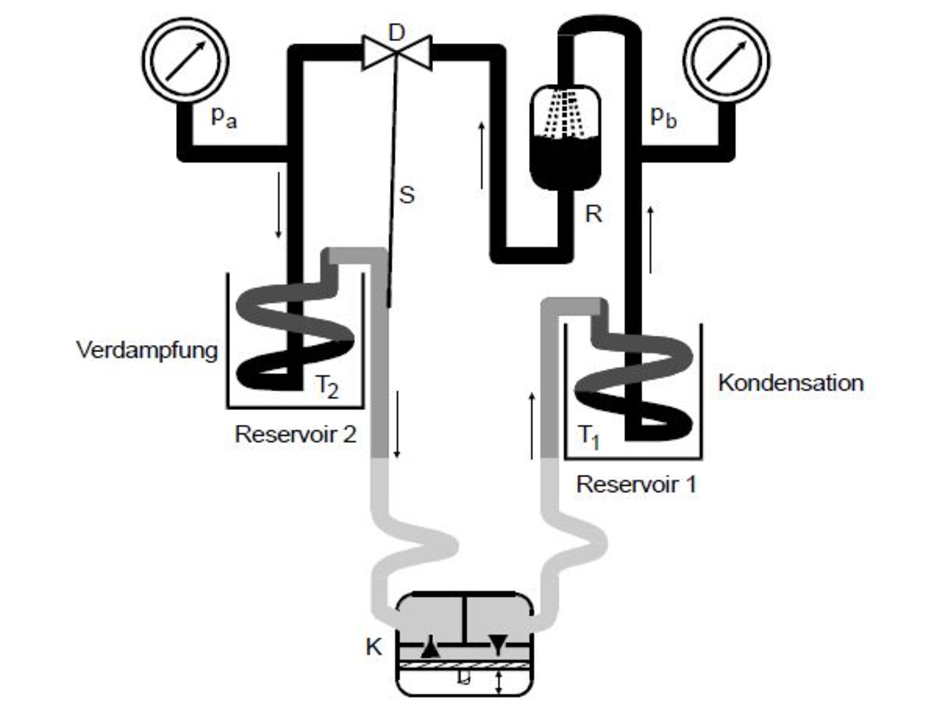
\includegraphics[scale=0.75]{aufbau_1.pdf}
               \caption{Prinzipieller Aufbau einer Wärmepumpe ($p_\text{b}$ > $p_\text{a}$; $T_1$ > $T_2$)}
               \label{fig:prinzW}
        \end{figure}
        Der Kompressor K erzeugt eine annähernd adiabatische Kompression, also eine Kompression ohne Wärmeverluste an die Umgebung. 
        Zusätzlich wird durch diese Kompression ein Mediumskreislauf im System ingang gebracht. Durch das Drosselventil D und dem hohen Strömungswiderstand baut sich ein Druckunterschied
        zwischen dem Eingang des Ventils und dessen Ausgang auf ($p_\text{b}-p_\text{a}$).

        Die Apparatur ist so konzipiert, dass das Gas Reservoir 2 und 1 durchströmt und jeweils sein Zustand in einem der beiden ändert. Dies bedeutet, dass das Gas sich im Reservoir 2 
        vergasförmigt und in Reservoir 1 durch den erhöhten Druck ($p_\text{b}$) wieder verflüssigt und so seine, durch die Vergasung, aufgenommene Wärme wieder abgibt. Die Messgröße der 
        Verdampfungswärme ist L pro Gramm Substanz.  Somit ist das Reservoir 1 das wärmere und Reservoir 2 das kältere.

        Damit die Apparatur störungsfrei arbeiten kann ist es notwendig weitere Armaturen ins System zu integrieren. Diese haben jedoch keinen direkten Einfluss auf die prinzipielle Wirkungsweise. 
        So benutzt man einen sogennanten "`Reiniger"' R, welches das verflüssigte Transportmedium von Gasblasen reinigt, sodass eine blasenfreie Flüssigkeitszufuhr zum Drosselventil D gewährleistet werden kann.
        Zudem wird eine "`Steuerungsvorrichtung"' S für das Drosselventil benutzt, sodass die Durchlässigkeit der Drosselventils über die Temperaturdifferenz zwischen Eingang und Ausgang ($T_2 - T_1$) 
        des Reservoirs 2 gesteuert werden kann.

    %4
    \newpage
    \section{Durchführung}
    Der Versuchsbau ist folgendermaßen:
    \begin{figure}
               \centering
               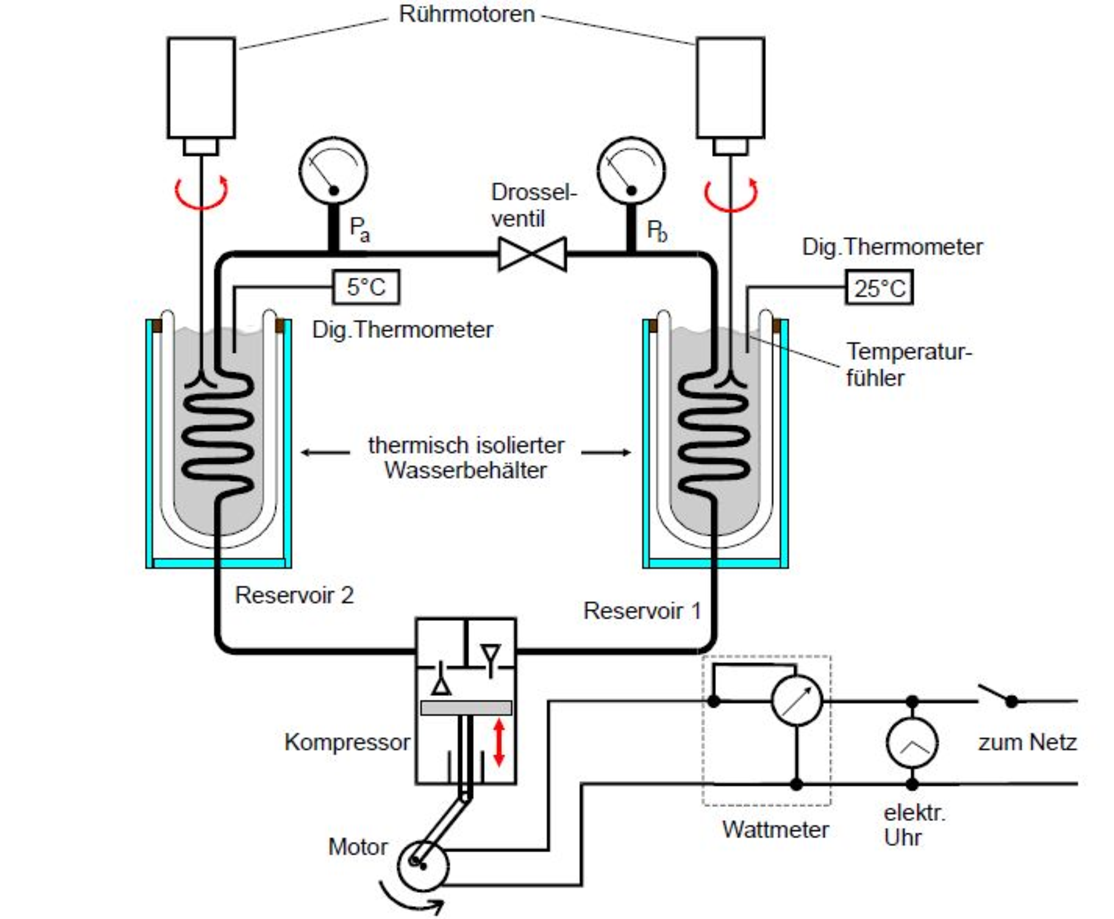
\includegraphics[width=\textwidth]{aufbau_2.pdf}
               \caption{Schematische Darstellung der kompletten Messapparatur}
               \label{fig:scheW}
    \end{figure}

    Sobald der Kompressor eingeschaltet wird, werden die Temperaturen T1 und T2, die Drücke p1 und p2 und die Kompressorleistung N an den Anzeigegeräten abgelesen. Damit die Zeitabstände
    beim Ablesen möglichst gleich sind, werden die Größen immer in derselben Reihenfolge notiert. Um die Drücke p1 und p2 zu erhalten, muss noch 1 bar auf die gemessenen Drücke p*1 und p*2 addiert werden.
